%% abtex2-modelo-trabalho-academico.tex, v-1.7.1 laurocesar
%% Copyright 2012-2013 by abnTeX2 group at http://abntex2.googlecode.com/ 
%%
%% This work may be distributed and/or modified under the
%% conditions of the LaTeX Project Public License, either version 1.3
%% of this license or (at your option) any later version.
%% The latest version of this license is in
%%   http://www.latex-project.org/lppl.txt
%% and version 1.3 or later is part of all distributions of LaTeX
%% version 2005/12/01 or later.
%%
%% This work has the LPPL maintenance status `maintained'.
%% 
%% The Current Maintainer of this work is the abnTeX2 team, led
%% by Lauro César Araujo. Further information are available on 
%% http://abntex2.googlecode.com/
%%
%% This work consists of the files abntex2-modelo-trabalho-academico.tex,
%% abntex2-modelo-include-comandos and abntex2-modelo-references.bib
%%

% ------------------------------------------------------------------------
% ------------------------------------------------------------------------
% abnTeX2: Modelo de Trabalho Academico (tese de doutorado, dissertacao de
% mestrado e trabalhos monograficos em geral) em conformidade com 
% ABNT NBR 14724:2011: Informacao e documentacao - Trabalhos academicos -
% Apresentacao
% ------------------------------------------------------------------------
% ------------------------------------------------------------------------

%%%%%%%%%%%%%%%%%%%%%%%%%%%%%%%%%%%%%%%%%%%%%%%%%%%%%%%%%%%%%%%%%%%%%%%%%%
% Alterações de layout realizadas no modelo do centro de informática da UFPE, abaixo informações sobre.
%
% Matheus Jonatha <mthsjonatha@gmail.com>
%
% Versão de dezembro de 2020 (1.0)
%
%%%%%%%%%%%%%%%%%%
%
% As alterações realizadas no leiaute original do abntex2 disponibilizado 
% no sharelatex adaptaram o leiaute do abntex2 aos requisitos mínimos
% para escrita de dissertações e teses customizadas para o 
% centro de informática da ufpe.
%
% Bruno Maciel <bifm@cin.ufpe.com> 20/10/2016
% Daniel Severo Estrázulas <dse@cin.ufpe.br> 19/10/2020
% Alterações realizadas para o template da biblioteca atualizado disponibilizado no site Versão 07.10.2020 (1.3) revisado pelas bibliotecárias do setor bibccen.pt@ufpe.br
%%%%%%%%%%%%%%%%%%%%%%%%%%%%%%%%%%%%%%%%%%%%%%%%%%%%%%%%%%%%%%%

\documentclass[
	% -- opções da classe memoir --
	12pt,				% tamanho da fonte
	openright,			% capítulos começam em pág ímpar (insere página vazia caso preciso)
	oneside,			% para impressão em verso e anverso. Oposto a oneside
	a4paper,			% tamanho do papel. 
	% -- opções da classe abntex2 --
	chapter=TITLE,		% títulos de capítulos convertidos em letras maiúsculas
	section=TITLE,		% títulos de seções convertidos em letras maiúsculas
	%subsection=TITLE,	% títulos de subseções convertidos em letras maiúsculas
	%subsubsection=TITLE,% títulos de subsubseções convertidos em letras maiúsculas
	% -- opções do pacote babel --
	%english,			% idioma adicional para hifenização
	french,				% idioma adicional para hifenização
	spanish,			% idioma adicional para hifenização
%	brazil,				% o último idioma é o principal do documento
	english,
	brazil,
	]{abntex2/abntex2}
	\renewcommand{\baselinestretch}{1.5} %para customizar o espaço entre as linhas do texto

% -----------------------------------------------------------
% SETTINGS
% -----------------------------------------------------------

\usepackage{abntex2/abntex2-ifrn}

% \usepackage[noframe]{showframe}
% \usepackage{showframe}

%\overfullrule=4mm %para identificar onde existem os alertas de linhas grandes mal formatada pelo LaTex, basta comentar para não aparecer a barra lateral preta na linha em questão.

\renewcommand*\arraystretch{1.2} %para customizar o espaço entre as linhas das tabelas


\usepackage{pdfpages} %para incluir pdf como páginas

% -----------------------------------------------------------
% PACOTES
% -----------------------------------------------------------

\usepackage{float}
\usepackage{cmap}				% Mapear caracteres especiais no PDF
\usepackage{lmodern}			% Usa a fonte Latin Modern			
\usepackage[T1]{fontenc}		% Selecao de codigos de fonte.
% \usepackage[utf8]{inputenc}	% JÁ VEM POR PADRÃO A PARTIR DO TEXLIVE 2018% Codificacao do documento (conversão % automática dos acentos)
\usepackage{lastpage}			% Usado pela Ficha catalográfica
\usepackage{indentfirst}		% Indenta o primeiro parágrafo de cada seção.
%\usepackage{color}				% Controle das cores
\usepackage{graphicx}			% Inclusão de gráficos
\usepackage{lipsum}				% para geração de dummy text
\usepackage[versalete,alf,abnt-and-type=e,abnt-etal-list=0,abnt-etal-cite=3]{abntex2/abntex2cite} 
\usepackage{multirow}
\usepackage[section]{placeins}
\usepackage{substr}


% -----------------------------------------------------------
% lista de abreviaturas e siglas
% início
% -----------------------------------------------------------
% \usepackage[noredefwarn,acronym]{glossaries} %GLOSSÁRIO
\usepackage[acronym,nonumberlist,nogroupskip,noredefwarn]{glossaries}
% \usepackage{glossary-superragged}

\newcolumntype{L}[1]{>{\raggedright\let\newline\\\arraybackslash\hspace{0pt}}m{#1}}
\newcolumntype{C}[1]{>{\centering\let\newline\\\arraybackslash\hspace{0pt}}m{#1}}
\newcolumntype{R}[1]{>{\raggedleft\let\newline\\\arraybackslash\hspace{0pt}}m{#1}}

\newglossarystyle{modsuper}{%
  \glossarystyle{super}%
  \renewcommand{\glsgroupskip}{}
  
  % put the glossary in a longtable environment:
 \renewenvironment{theglossary}%
  {
    \begin{longtable}
        {L{0.2\textwidth}L{0.8\textwidth}}}%
    {\end{longtable}
  }%
}

% -----------------------------------------------------------
% lista de abreviaturas e siglas
% fim
% -----------------------------------------------------------

\usepackage{lscape} 
\usepackage{rotating} %rotates the figures, page
\usepackage{tikz}
\usepackage[section]{placeins}
\usepackage{setspace} 

% ----------------------------------------------------------
% PERSONALIZAÇÃO DE CORES
% ----------------------------------------------------------

\definecolor{blue}{RGB}{41,5,195}
\definecolor{gray}{rgb}{.4,.4,.4}
\definecolor{gray}{rgb}{.4,.4,.4}
\definecolor{pblue}{rgb}{0.13,0.13,1}
\definecolor{pgreen}{rgb}{0,0.5,0}
\definecolor{pred}{rgb}{0.9,0,0}
\definecolor{pgrey}{rgb}{0.46,0.45,0.48}
\definecolor{lightgray}{rgb}{0.95, 0.95, 0.96}
\definecolor{whitesmoke}{rgb}{0.96, 0.96, 0.96}
\definecolor{javared}{rgb}{0.6,0,0} % for strings
\definecolor{javagreen}{rgb}{0.25,0.5,0.35} % comments
\definecolor{javapurple}{rgb}{0.5,0,0.35} % keywords
\definecolor{javadocblue}{rgb}{0.25,0.35,0.75} % javadoc
\definecolor{meucinza}{rgb}{0.5, 0.5, 0.5}
%\definecolor{lightgray}{gray}{0.9}


% ----------------------------------------------------------
% PERSONALIZAÇÃO DO USUÁRIO
% ----------------------------------------------------------

% ----------------------------------------------------------
% DADOS DO TRABALHO - CAPA e FOLHA DE ROSTO
% Configure os dados do trabalho aqui
% ----------------------------------------------------------
\instituicao{INSTITUTO FEDERAL DE EDUCAÇÃO, CIÊNCIA E TECNOLOGIA \\ DO RIO GRANDE DO NORTE}
\autor{NOME COMPLETO DO (A) AUTOR (A)}
\titulo{\textbf{TÍTULO DO TRABALHO: SUBTÍTULO}}
\local{NATAL}
\data{\Year}

% ----------------------------------------------------------

\departamento{DIAC}
\programa{Graduação}
\emailprograma{mthsjonatha@gmail.com}
\siteprograma{mthsjonatha.github.io}
\tipotrabalho{Dissertação de Licenciatura}
%\areaconcentracao{\textbf{Área de Concentração}: Texto Texto}
\orientador{Orientador (a): Nome Aqui}
\coorientador{Coorientador (a): Nome Aqui}

% ----------------------------------------------------------

\preambulo{Trabalho de Conclusão de Curso apresentado ao Curso Xxxxxxxxxxxxxxxxxxxxxxxxxxxxxxxxxxxx xxxxxxxxxxxxxxxxxxxxxxxx do Instituto Federal de Educação, Ciência e Tecnologia do Rio Grande do Norte, em cumprimento às exigências legais como requisito parcial à obtenção do título de Xxxxxxxxxxxxxx.}

\preambuloatadefesa{Dissertação apresentada ao Programa de Pós-Graduação Profissional em Ciência da Computação da Universidade Federal de Pernambuco, como requisito parcial para a obtenção do título de Mestre Profissional em 04 de setembro de 2020.}


% ----------------------------------------------------------
% COMPILA O ÍNDICE
% ----------------------------------------------------------

\makeindex

% ----------------------------------------------------------
% LISTA E ABREVIATURAS E SIGLAS
% ----------------------------------------------------------

%lista de siglas
\newacronym{MEC}{MEC}{Ministerio da Educação e Cultura} % TIRAR DEPOIS
\newacronym{UFPE}{UFPE}{UNIVERSIDADE} % TIRAR DEPOIS
\newacronym{ABNT}{ABNT}{Associação Brasileira de Normas Técnicas}
\newacronym{BCSF}{BCSF}{Instituto Brasileiro de Geografia e Estatística}
\newacronym{IBGE}{IBGE}{Biblioteca Central Sebastião Fernandes}
\newacronym{NBR}{NBR}{Norma Brasileira Regulamentar}
\newacronym{PUCPR}{PUCPR}{Pontifícia Universidade Católica do Paraná}
\newacronym{SIBI}{SIBI}{Biblioteca Central Sebastião Fernandes}
\newacronym{trad.}{trad.}{Tradutor}


\makenoidxglossaries
\renewcommand*{\glsseeformat}[3][\seename]{\textit{#1}  
\glsseelist{#2}}

\renewcommand*{\glspostdescription}{} % remove trailing dot
\renewcommand{\glsnamefont}[1]{\textbf{#1}}

\renewcommand{\familydefault}{\sfdefault}

% ----------------------------------------------------------
% GLOSSÁRIO
% ----------------------------------------------------------


\newglossaryentry{naive-bayes}
{
  name=\textit{Na{\"i}ve Bayes},
  description={},
  plural=\textit{Na{\"i}ve Bayes}
}

\newglossaryentry{hoeffding-tree}
{
  name=\textit{Hoeffding Tree},
  description={},
  plural=\textit{Hoeffding Trees}
}













\usepackage{pdfpages}
\usepackage{inconsolata}
\usepackage{listings}

\definecolor{cinza}{HTML}{FCF8F8}

% define formato e estilo dos elementos do tipo Codigo Fonte
\lstset{language=PHP,
basicstyle=\ttfamily\scriptsize,
%basicstyle=\ttfamily,
keywordstyle=\color{javapurple}\bfseries,
stringstyle=\color{pblue},
commentstyle=\color{javagreen},
morecomment=[s][\color{javadocblue}]{/**}{*/},
morecomment=[s][\color{gray}]{@}{\ },
numbers=left,
numberstyle=\tiny\color{black},
backgroundcolor=\color{cinza},
stepnumber=2,
numbersep=8pt,
xleftmargin=14pt,
tabsize=4,
showspaces=false,
showstringspaces=false,
breaklines=true,}

%%%%%%%%%%%%%%%%%%%%%%%%%%%%%%%%%%



\usepackage{adjustbox} % ajustar tabela ao tamanho da pagina

% ----------------------------------------------------------
% INÍCIO DO DOCUMENTO
% ----------------------------------------------------------

\begin{document}

\frenchspacing % Retira espaço extra obsoleto entre as frases.

\imprimircapa
\imprimirfolhaderosto*~
%a ficha deve ser passada pelo setor da biblioteca e sobrescrito no formato pdf

\includepdf[pages=-]{ElementosPreTextuais/ficha.pdf}

%\newpage
%\input{ElementosPreTextuais/ata_defesa}
%a folha de aprovação deve ser um pdf que a secretaria encaminha sem assinaturas
%basta fazer upload na basta others e sobrescrever

\includepdf[pages=-]{others/folha_aprovacao_original}

% ----------------------------------------------------------
% DEDICATÓRIA
% ----------------------------------------------------------
\begin{dedicatoria}
   \vspace*{\fill}
%   \centering
  % \noindent
   %\textit{\lipsum[2]} 
   Dedicatória
   %\vspace*{\fill}
\end{dedicatoria}
% ---

% ----------------------------------------------------------
% AGRADECIMENTOS
% ----------------------------------------------------------
\begin{agradecimentos}
É um elemento opcional, inserido após a dedicatória. Trata-se de um texto em que o autor faz agradecimentos dirigidos àqueles que contribuíram de maneira relevante à elaboração do trabalho. Segue a mesma tipologia das seções primárias.

À CAPES, pelo apoio financeiro com a manutenção da bolsa de auxílio.

Ao Prof. Dr. Xxxxx Xxxxx Xxxxx, pela excelente orientação.

Aos professores participantes da banca examinadora Xxxxx Xxxxx Xxxxx e Xxxxx Xxxxx Xxxxx pelo tempo, pelas valiosas colaborações e sugestões.

Aos professores entrevistados, pelo tempo concedido nas entrevistas.

Aos colegas da turma do curso, pelas reflexões, críticas e sugestões recebidas.




\end{agradecimentos}


% ----------------------------------------------------------
% EPÍGRAFE

%Epígrafe: Elemento opcional e sem título em que o (a) autor (a) apresenta uma citação relacionada ao assunto tratado no trabalho. Deve ser elaborada conforme a ABNT-NBR 10520 (Citações). As citações de até três linhas devem estar entre aspas duplas e as citações com mais de três linhas devem ser destacadas com recuo de 4 cm da margem esquerda, com letra menor que a do texto e sem as aspas. A fonte da citação deve aparecer na lista de referências.
% ---------------------------------------------------------
\vspace*{10cm}
%\begin{citacao}
%Citação relacionada com o tema do trabalho, com indicação de autoria. Sobrenome do autor \cite{manualufpe2020}.
%\end{citacao}

    % \vspace*{5cm}
\begin{epigrafe}	
		Citação relacionada com o tema do trabalho, com indicação de autoria. Sobrenome do autor \cite[p. 4]{manualufpe2020}.
\end{epigrafe}
	





% resumo em português
\begin{resumo}[Resumo] 
Trata-se de um elemento obrigatório. O título da seção (Resumo) deve ser centralizado e em negrito. A primeira frase deve ser significativa e relacionada ao tema. Deve apresentar os aspectos mais relevantes do trabalho, como objetivos, metodologia, resultados e conclusões. Usa-se o verbo na voz ativa e na terceira pessoa do singular. Evitar símbolos, contrações, fórmulas, equações, diagramas e recomenda-se evitar citações. Conforme a NBR 6028, a extensão do resumo deve conter de 150 a 500 palavras, dispostas em parágrafo único sem recuo e com espaçamento 1,5 entre linhas. Em seguida, deve-se indicar as palavras-chave, que devem ser separadas entre si por ponto e finalizadas também por ponto. 

% \noindent %- o resumo deve ter apenas 1 parágrafo e sem recuo de texto na primeira linha, essa tag remove o recuo. Não pode haver quebra de linha.

 \vspace{\onelineskip}
    
 \noindent
 \textbf{Palavras-chaves}: Palavra 1. Palavra 2. Palavra 3.
\end{resumo}



% resumo em inglês
\begin{resumo}[Abstract]
\begin{otherlanguage*}{english}

 %\noindent
Trata-se de uma versão do resumo para idioma de divulgação internacional. É um elemento obrigatório. Deve seguir os mesmos padrões do resumo na língua vernácula, conforma a NBR 6028. 



   \vspace{\onelineskip} 
 
   \noindent 
   \textbf{Keywords}: Palavra 1. Palavra 2. Palavra 3.
 \end{otherlanguage*}
 \end{resumo}



% ----------------------------------------------------------
% LISTA DE FIGURAS
% ----------------------------------------------------------

\pdfbookmark[0]{\listfigurename}{lof}
\listoffigures*
\cleardoublepage

% ----------------------------------------------------------
% LISTA DE CÓDIGOS FONTES
% ----------------------------------------------------------

\pdfbookmark[0]{\lstlistingname}{lol} % caso não tenha quadros, comente esta linha 
\counterwithout{lstlisting}{chapter}



% Altera o nome padrão do rótulo usado no comando \autoref{}
\renewcommand{\lstlistingname}{Código Fonte}

% Altera o rótulo a ser usando no elemento pré-textual "Lista de código"
\renewcommand{\lstlistlistingname}{Lista de códigos}

% Configura a ``Lista de Códigos'' conforme as regras da ABNT (para abnTeX2)
\begingroup\makeatletter
\let\newcounter\@gobble\let\setcounter\@gobbletwo
  \globaldefs\@ne \let\c@loldepth\@ne
  \newlistof{listings}{lol}{\lstlistlistingname}
  \newlistentry{lstlisting}{lol}{0}
\endgroup

\renewcommand{\cftlstlistingaftersnum}{\hfill--\hfil}

\let\oldlstlistoflistings\lstlistoflistings
{
\let\oldnumberline\numberline
\newcommand{\algnumberline}[1]{Código Fonte~#1~\enspace--~\enspace}
\renewcommand{\numberline}{\algnumberline}

\begin{KeepFromToc}
\lstlistoflistings
\end{KeepFromToc}
}
\cleardoublepage


% ----------------------------------------------------------
% LISTA DE QUADROS
% ----------------------------------------------------------

\pdfbookmark[0]{\listofquadrosname}{loq} % caso não tenha quadros, comente esta linha 
\listofquadros* % caso não tenha quadros, comente esta linha 
\cleardoublepage

% ----------------------------------------------------------
% LISTA DE TABELAS
% ----------------------------------------------------------

\pdfbookmark[0]{\listtablename}{lot}
\listoftables*
\cleardoublepage

% ----------------------------------------------------------
% LISTA E ABREVIATURAS E SIGLAS
% ----------------------------------------------------------
% \printglossary[type=\acronymtype,title={\listadesiglasname},nonumberlist]
% \printglossaries
% compile uma vez com o comando \printglossaries e depois compile novamente com o comando \printglossaries comentado para as páginas glossário e siglas serem ocultadas.

% ----------------------------------------------------------
% LISTA E ABREVIATURAS E SIGLAS
% ----------------------------------------------------------
% \setglossarystyle{modsuper}
\printnoidxglossary[style=modsuper,type=\acronymtype,title={\listadesiglasname},nonumberlist]
% \printglossary[style=super, type=\acronymtype]
\cleardoublepage



% ----------------------------------------------------------
% LISTA DE SIMBOLOS
% ----------------------------------------------------------




% ---

% ---
% inserir lista de símbolos
% ---
\begin{simbolos}
  \item[$ \gamma $] Letra grega Gama
  %\item[$ \Lambda $] Lambda
  %\item[$ \zeta $] Letra grega minúscula zeta
  \item[$ \in $] Pertence
%  \item[$ \infty$] Infinito
%  \item[$ \ge$] Maior ou Igual
  \item[$ \delta$] Delta
  \item[$ \theta$] Teta
  \item[$ \sigma$] Sigma
  \item[$ \mu$] Mi
  
\end{simbolos}
% ---




% ----------------------------------------------------------



% ----------------------------------------------------------
% SUMÁRIO
% ----------------------------------------------------------
\pdfbookmark[0]{\contentsname}{toc}
\tableofcontents*
% \begingroup\intoctrue
% \tableofcontents*
% \endgroup
\cleardoublepage

% \setcounter{page}{13}
\setcounter{tocdepth}{2}
\setcounter{table}{0}



% ----------------------------------------------------------
% IMPORTANDO ELEMENTOS E CAPÍTULOS
% ----------------------------------------------------------

% AQUI VOCÊ CONTROLA QUAIS ELEMENTOS E CAPÍTULOS DEVEM SER EXIBIDOS, RECOMENDADO DESATIVAR AS ETAPAS QUE JÁ FORAM CONCLUÍDAS, ASSIM O ARQUIVO É COMPILADO MAIS RÁPIDO.
% os elementos pré-textuais devem ser modificados no main.tex
% o titulo, autor,instituição  e outros dados, devem ser informados no arquivo dadoDoTrabalho.tex

%%%%%%%%%%%%%%%%%%%%%%%%%%%%%%%%%%%%%%%%%%%%%%%%%%%%%%%%
% ELEMENTOS TEXTUAIS
%%%%%%%%%%%%%%%%%%%%%%%%%%%%%%%%%%%%%%%%%%%%%%%%%%%%%%%%
% ------------------------------------------------------
% introdução
% ------------------------------------------------------
\textual
	% exemplo de organização interna de um capítulo separando por mais de um arquivo

\chapter{Introdução}
\label{chap:introducao}
Esta é a primeira seção textual do trabalho onde se deve apresentar ideias, delimitando o assunto, bem como o objetivo geral e específico da pesquisa e outros. Elemento necessário para situar acerca da estrutura do trabalho.

Todo texto deve ser digitado em fonte times new roman ou arial, tamanho 12, inclusive a capa, com exceção das citações com mais de três linhas, notas de rodapé, paginação, dados internacionais de catalogação-na-publicação (ficha catalográfica), legendas e fontes das ilustrações e das tabelas, que devem ser em fonte times new roman ou arial, tamanho menor (10 ou 11). O texto deve ser justificado, exceto as referências, no final do trabalho, que devem ser alinhadas a esquerda.

Todos os autores citados devem ter a referência incluída em lista no final no trabalho.


 
 
\chapter{Texto Texto Texto}
\label{chap:intro}


 Texto \textit{text} texto texto texto texto texto texto texto texto texto texto texto texto texto texto texto texto texto texto texto texto texto texto texto texto texto texto texto texto texto texto texto texto texto texto texto, no \gls{MEC}.

 Segundo \citeonline{manualufpe2020}, o \gls{MEC}, texto texto texto texto texto texto texto texto texto texto texto texto texto texto texto texto texto texto texto texto texto texto texto texto texto texto texto texto texto texto texto texto texto texto texto texto .
 
 \begin{citacao}
 Texto \textit{text} texto texto texto texto texto texto texto texto texto texto texto texto texto texto texto texto texto texto texto texto texto texto texto texto texto texto texto texto texto texto texto texto texto texto texto texto texto texto texto texto texto \cite{manualufpe2020}.  
 \end{citacao}


 
 
\section{Texto Texto Texto}
\label{motivacao}

Texto texto texto texto texto texto texto texto texto texto texto texto texto texto texto texto texto texto texto texto texto texto texto texto texto texto texto texto texto texto texto texto texto texto texto texto, \textbf{exemplo} sigla \gls{SIBI}.

\input{ElementosTextuais/imagens/captitulo1/figuraex}

Texto texto texto texto texto texto texto texto texto texto texto texto texto texto texto texto texto texto texto texto texto texto texto texto texto texto texto texto texto texto texto texto texto texto texto texto, conforme Figuras \ref{fig:figuraex} e Figuras \ref{fig:figuraex2}, continua no Capítulo %\ref{chap:outrocapitulo}.


\input{ElementosTextuais/imagens/captitulo1/figuraex2}

Texto texto texto texto texto texto texto texto texto texto texto texto texto texto texto texto texto texto texto texto texto texto texto texto texto texto texto \gls{UFPE}.

%\input{ElementosTextuais/Introducao/Capitulos/problemahipotese.tex}
\section{Texto Texto Texto}
\label{objetivos}
Texto texto texto texto texto texto texto texto texto texto texto texto texto texto texto texto texto texto texto texto texto texto texto texto texto texto texto texto texto texto texto texto texto texto texto texto.

Texto texto texto texto texto texto texto texto texto texto texto texto texto texto texto texto texto texto texto texto texto texto texto texto texto texto texto texto texto texto texto texto texto texto texto texto.

\subsection{Texto Texto Texto}
\label{sub:exemplonivel3}

Texto texto texto texto texto texto texto texto texto texto texto texto texto texto texto texto texto texto texto texto texto texto texto texto texto texto texto texto texto texto texto texto texto texto texto texto.

\subsubsection{Texto texto texto texto}
\label{subsub:exemplonivel4}

Texto texto texto texto texto texto texto texto texto texto texto texto texto texto texto texto texto texto texto texto texto texto texto texto texto texto texto texto texto texto texto texto texto texto texto texto.
%\input{ElementosTextuais/Introducao/Capitulos/organizacao.tex}
	\chapter{Texto Texto Texto}
\label{chap:outrocapitulo}

Texto texto texto texto ''texto'' texto texto texto texto texto texto texto texto texto texto texto texto texto texto texto texto texto texto texto texto texto texto texto texto texto texto texto texto texto texto texto, confome Tabela \ref{tbl:tabelaex} e a Tabela \ref{tbl:tabelaex2}.

%exemplo de inputs, ideal para organização e troca de posicionamento futuro é ter um elemento por arquivo

%usar um gerador é uma opção https://www.tablesgenerator.com/
% observação, segundo a biblioteca tableas não podem ter nenhuma linha vertical

\begin{table}[ht]
\caption{Texto Texto Texto}
\label{tbl:tabelaex}
\centering
\rowcolors{1}{}{lightgray}
\begin{tabular}{p{6cm}p{9cm}}
\hline
\multicolumn{1}{c}{\textbf{Coluna A}} & \multicolumn{1}{c}{\textbf{Coluna B}}  \\
\hline     
\textbf{coluna1} & Texto Texto Texto Texto Texto Texto Texto Texto Texto Texto Texto Texto.
\\ 

coluna2 & Texto Texto Texto Texto Texto Texto Texto Texto Texto Texto Texto Texto.              
\\ 

coluna3 & Texto \textit{Texto} Texto Texto Texto Texto Texto Texto Texto Texto Texto Texto.     
\\ \hline

\end{tabular}

  \par\medskip\ABNTEXfontereduzida\selectfont\textbf{Fonte:} Elaborada pelo autor (2020) \par\medskip
\end{table}



%usar um gerador é uma opção https://www.tablesgenerator.com/
% observação, segundo a biblioteca tableas não podem ter nenhuma linha vertical

\begin{table}[ht]
\caption{Texto Texto Texto}
\label{tbl:tabelaex2}
\centering
\rowcolors{1}{}{lightgray}
\begin{tabular}{p{6cm}p{9cm}}
\hline
\multicolumn{1}{c}{\textbf{Coluna A}} & \multicolumn{1}{c}{\textbf{Coluna B}}  \\
\hline 
coluna1 & Texto Texto Texto Texto Texto Texto ''Texto'' Texto Texto Texto Texto Texto.
\\ 

coluna2 & Texto Texto Texto Texto Texto Texto Texto Texto Texto Texto Texto Texto.              
\\

coluna3 & Texto \textit{Texto} Texto Texto Texto Texto Texto Texto Texto Texto Texto Texto.     
\\ \hline

\end{tabular}

  \par\medskip\ABNTEXfontereduzida\selectfont\textbf{Fonte:} \citeauthor{manualufpe2020} (\citeyear{manualufpe2020}) \par\medskip
\end{table}


\section{Texto Texto}
\label{sec:section}

Texto texto texto texto ''texto'' texto texto texto texto texto texto texto texto texto texto texto texto texto texto texto texto texto texto texto texto texto texto texto texto texto texto texto texto texto texto texto \cite{gil2002elaborar}.


\section{Texto Texto}
\label{sec:outrasection}

Texto texto texto texto ''texto'' texto texto texto texto texto texto texto texto texto texto texto texto texto texto texto texto texto texto texto texto texto texto texto texto texto texto texto texto texto texto texto

\subsection{Texto Texto Texto}
\label{sub:outrasubsectiona}

Texto texto texto texto ''texto'' texto texto texto texto texto texto texto texto texto texto texto texto texto texto texto texto texto texto texto texto texto texto texto texto texto texto texto texto texto texto texto


\subsubsection{Texto Texto Texto Texto}
\label{subsub:outrasubsubsection}

Texto texto texto texto ''texto'' texto texto texto texto texto texto texto texto texto texto texto texto texto texto texto texto texto texto texto texto texto texto texto texto texto texto texto texto texto texto texto

\subsubsection{Texto Texto Texto Texto}
\label{subsub:outrasubsubsection2a}

Texto texto texto texto ''texto'' texto texto texto texto texto texto texto texto texto texto texto texto texto texto texto texto texto texto texto texto texto texto texto texto texto texto texto texto texto texto texto

%a organização fica a seu critério se preferir utilize inputs para cada seção, subseção etc...
%apenas um exemplo de subseção em arquivo para ser incluido
\subsection{Texto Texto Texto}
%\label{sub:outrasubsection2}

Texto texto texto texto ''texto'' texto texto texto texto texto texto texto texto texto texto texto texto texto texto texto texto texto texto texto texto texto texto texto texto texto texto texto texto texto texto texto


\subsubsection{Texto Texto Texto Texto}
%\label{subsub:outrasubsubsection2}

Texto texto texto texto ''texto'' texto texto texto texto texto texto texto texto texto texto texto texto texto texto texto texto texto texto texto texto texto texto texto texto texto texto texto texto texto texto texto

%apenas um exemplo de subseção em arquivo para ser incluido

\section{Texto Texto}
\label{sec:section3}

Texto texto texto texto ''texto'' texto texto texto texto texto texto texto texto texto texto texto texto texto texto texto texto texto texto texto texto texto texto texto texto texto texto texto texto texto texto texto
	\chapter{Texto Texto Texto}
%não se esqueça de definir uma label única para utilizar no comando \ref
%\label{chap:metodologia}

Texto texto texto texto texto texto texto texto texto texto texto texto texto texto texto texto texto texto texto texto texto texto texto texto texto texto texto texto texto texto texto texto texto texto texto texto.

%exemplos de parágrafos com footnote
Texto texto texto texto texto texto texto texto texto texto texto texto texto texto texto texto texto texto texto texto texto texto texto texto texto texto texto texto texto texto texto texto texto texto texto texto \textit{Footnote} \footnote{Segundo \citeonline{manualufpe2020}, Exemplo de nota de rodapé.}.

\section{Texto Texto}
%\label{sec:algumlabel}

Texto texto texto texto texto texto texto texto texto texto texto texto texto texto texto texto texto texto texto texto texto texto texto texto texto texto texto texto texto texto texto texto texto texto texto texto.

Texto texto texto texto texto texto texto texto texto texto texto texto texto texto texto texto texto texto texto texto texto texto texto texto texto texto texto texto texto texto texto texto texto texto texto texto \textit{Footnote} \footnote{Segundo \citeonline{manualufpe2020}, Exemplo de nota de rodapé 2.}.

%exemplo de código fonte, as configurações estão no arquivo packages.tex
\lstinputlisting[language=PHP, 
caption=Texto texto texto texto
,label=lst:exemplocodigo1]{ElementosTextuais/antigo/trechos_codigo/funcoescatdinamicas.m}

\hspace{4cm}
\hfill
\begin{minipage}[t]{.65\textwidth}
\ABNTEXfontereduzida\selectfont\textbf{Fonte:} Elaborado pelo autor (2020) 
\end{minipage}


Texto texto texto texto texto texto texto texto texto texto texto texto texto texto texto texto texto texto texto texto texto texto texto texto texto texto texto texto texto texto texto texto texto texto texto texto, referente ao Código Fonte \ref{lst:exemplocodigo1} função \texttt{nome\_funcao}.

\subsection{Texto Texto Texto}
\label{subsec:algumlabel}

Texto texto texto texto texto texto texto texto texto texto texto texto texto texto texto texto texto texto texto texto texto texto texto texto texto texto texto texto texto texto texto texto texto texto texto texto.

\section{Texto Texto}
\label{sec:algumlabel2}
%exemplo de quadro
Texto texto texto texto texto texto texto texto texto texto texto texto texto texto texto texto texto texto texto texto texto texto texto texto texto texto texto texto texto texto texto texto texto texto texto texto, ver Quadro \ref{quad:exemplo_de_quadro}.

%a diferença do quadro pra tabela é que o quadro tem linhas verticais
\begin{quadro}
\caption{Texto texto texto texto texto}
\label{quad:exemplo_de_quadro}
\centering
\begin{tabular}{|lllll|}
\cline{1-5}
A& B &  C& D &E  \\ \cline{1-5}
\multirow{3}{*}{1}  & 2 &  3& 4& 5 \\
 &  2 &  3& 4& 5  \\
 &  2 &  3& 4& 5 \\
 \cline{1-5}
\end{tabular}
  \par\medskip\ABNTEXfontereduzida\selectfont\textbf{Fonte:} Elaborada pelo autor (2020) \par\medskip
\end{quadro}


\subsection{Texto Texto Texto}
\label{subsec:algumlabel2}
Texto texto texto texto texto texto texto texto texto texto texto texto texto texto texto texto texto texto texto texto texto texto texto texto texto texto texto texto texto texto texto texto texto texto texto texto.

\subsection{Texto Texto Texto}
\label{subsec:algumlabel3}

Texto texto texto texto texto texto texto texto texto texto texto texto texto texto texto texto texto texto texto texto texto texto texto texto texto texto texto texto texto texto texto texto texto texto texto texto.

	\chapter{Texto Texto Texto}
%\label{chap:capitulo1}

Texto texto texto texto texto texto texto texto texto texto texto texto texto texto texto texto texto texto texto texto texto texto texto texto texto texto texto texto texto texto texto texto texto texto texto texto.


\lstinputlisting[language=Java, 
caption=Texto texto texto texto
,label=lst:exemplocodigo2]{ElementosTextuais/antigo/trechos_codigo/java.m}
\hfill
\begin{minipage}[t]{.65\textwidth}
\ABNTEXfontereduzida\selectfont\textbf{Fonte:} \citeauthor{universidadejava2020}  (\citeyear{universidadejava2020}) 
\end{minipage}




\section{Texto Texto Texto}
%\label{sec:label}
Texto texto texto texto texto texto texto texto texto texto texto texto texto texto texto texto texto texto texto texto texto texto texto texto texto texto texto texto texto texto texto texto texto texto texto texto, ver Capítulo %\ref{chap:metodologia}, Seção \ref{sec:algumlabel}.

Texto texto texto texto texto texto texto texto texto texto texto texto texto texto texto texto texto texto texto texto texto texto texto texto texto texto texto texto texto texto texto texto texto texto texto texto (Código Fonte %\ref{lst:exemplocodigo2}).


\section{Texto Texto}
%\label{sec:outralabel}

Texto texto texto texto texto texto texto texto texto texto texto texto texto texto texto texto texto texto texto texto texto texto texto texto texto texto texto texto texto texto texto texto texto texto texto texto.


\bookmarksetup{startatroot}% 
% ------------------------------------------------------
% desenvolvimento
% ------------------------------------------------------

% ------------------------------------------------------
% conclusão
% ------------------------------------------------------


%%%%%%%%%%%%%%%%%%%%%%%%%%%%%%%%%%%%%%%%%%%%%%%%%%%%%%%%
% ELEMENTOS PÓS-TEXTUAIS
%%%%%%%%%%%%%%%%%%%%%%%%%%%%%%%%%%%%%%%%%%%%%%%%%%%%%%%%
\postextual

% ----------------------------------------------------------
% Referências bibliográficas
% ----------------------------------------------------------
%\bibliographystyle{abntexalfenglish} %caso seja em inglês, retire o comentário desta linha
% \renewcommand{\bibname}{REFER\^ENCIAS}
%\renewcommand{\bibname}{Bibliography}
% \addbibresource{mendeley.bib}
\bibliography{referencias}

% ------------------------------------------------------
% ademais
% ------------------------------------------------------
	

% ----------------------
% força para que não exiba subtítulos em apêndices no sumário
% -----------------------

\begin{apendicesenv}
\addtocontents{toc}{\protect\setcounter{tocdepth}{1}}
\makeatletter
\addtocontents{toc}{%
  \begingroup
  \let\protect\l@chapter\protect\l@section
  \let\protect\l@section\protect\l@subsection
}
\makeatother

% Imprime uma página indicando o início dos apêndices
% \partapendices

%coloca o identificador do anexo/apendice somente na primeira página
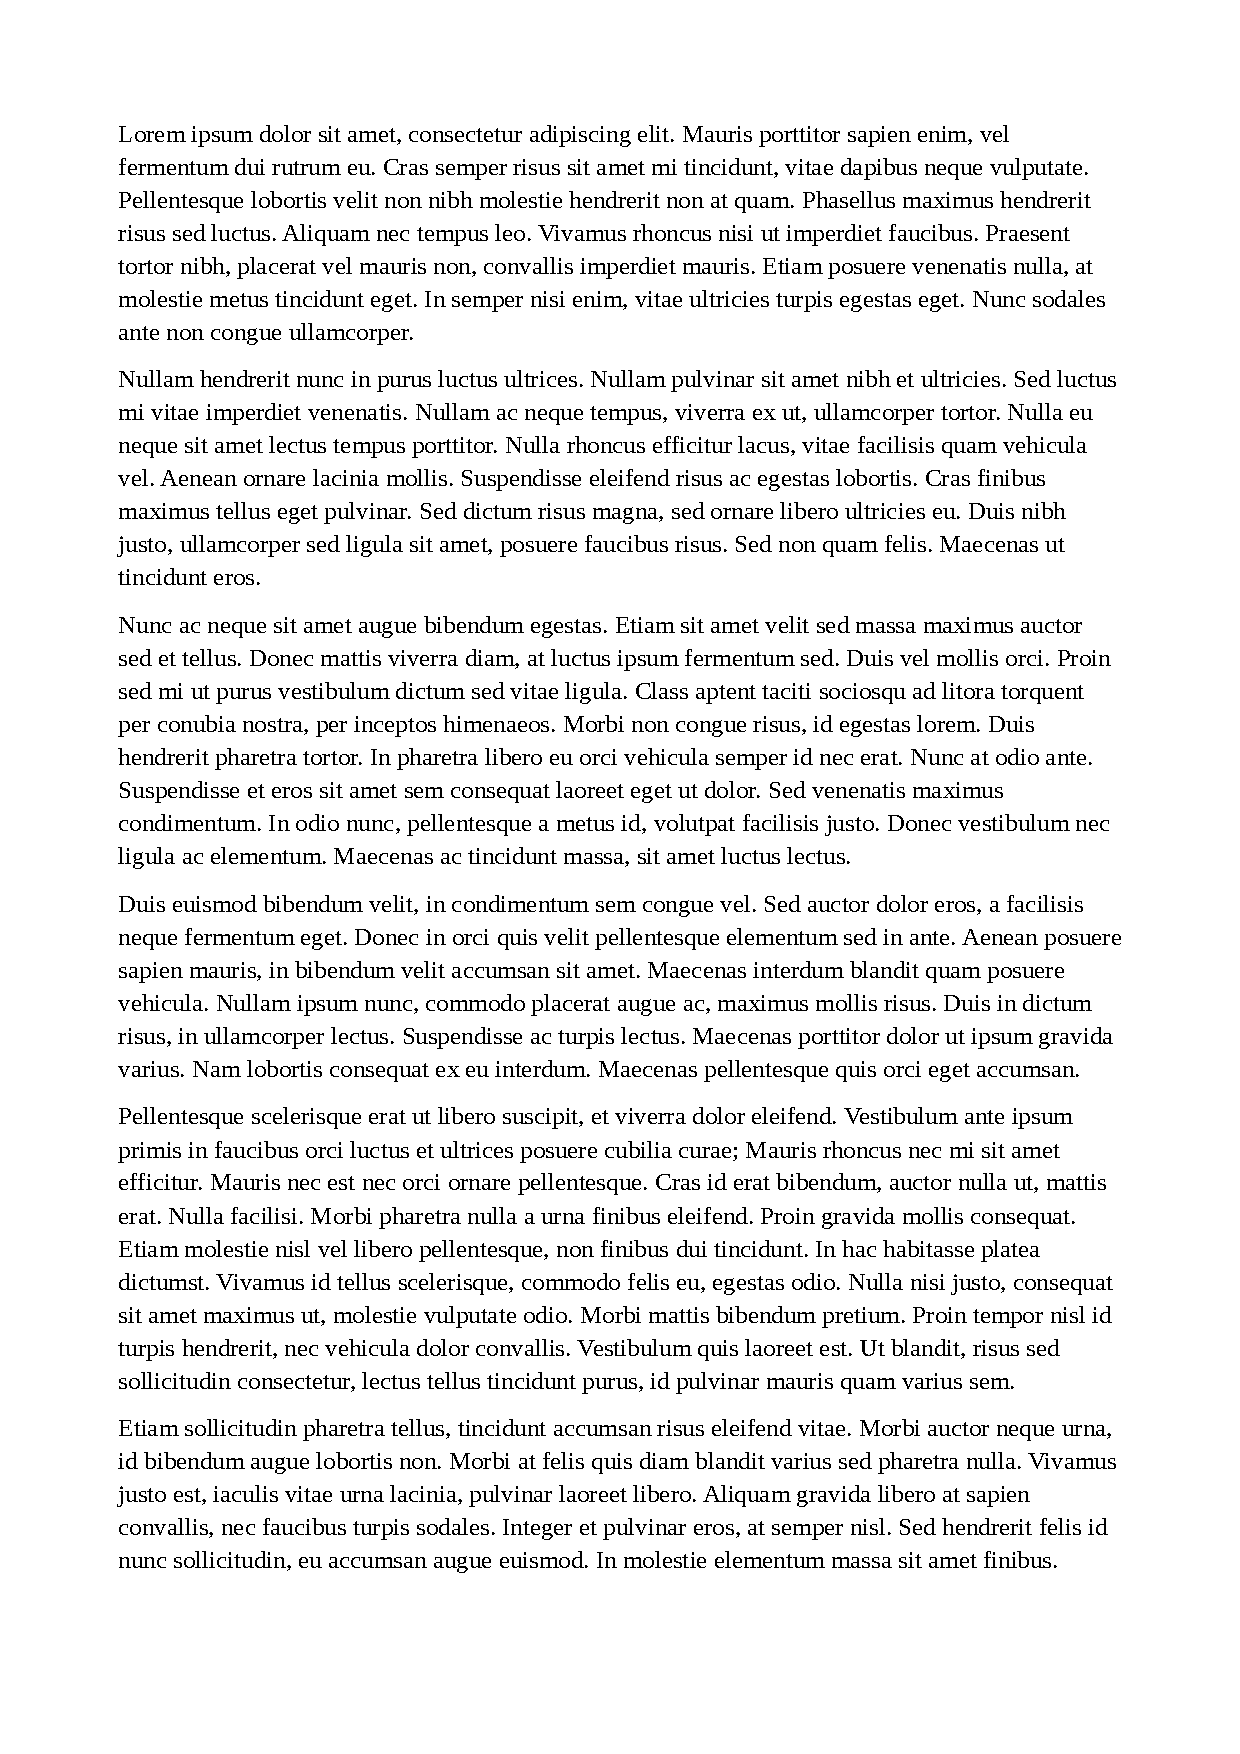
\includepdf[pages={1},scale=0.8,pagecommand=\chapter{Texto Texto Texto Texto}\label{apen:apendiceA}]{appendix/apendiceA}
\includepdf[pages={2-},scale=0.80,pagecommand={}]{appendix/apendiceA}

%coloca o identificador do anexo/apendice somente na primeira página
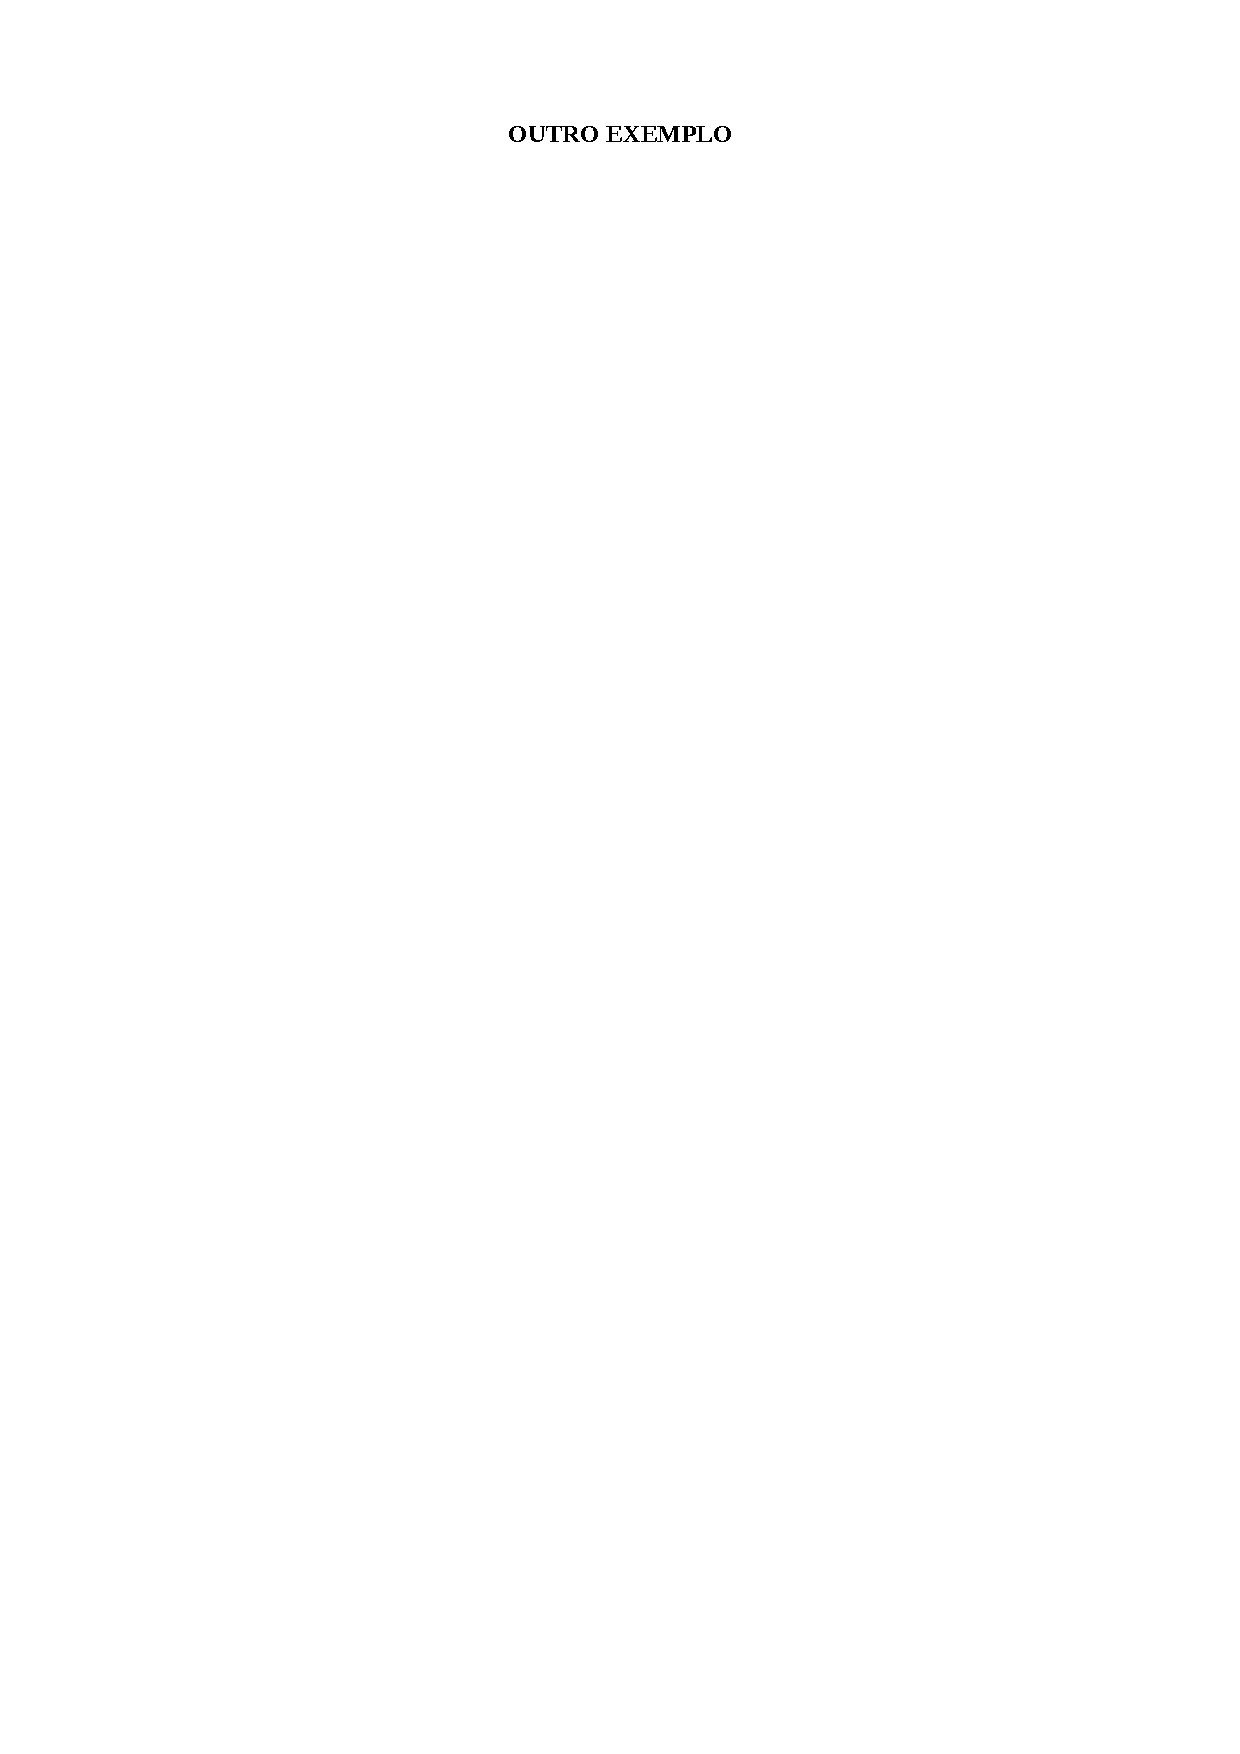
\includepdf[pages={1},scale=0.80,pagecommand=\chapter{Texto Texto Texto}\label{apen:apendiceB}]{ElementosPosTextuais/Apendice/apendiceB}


%coloca o identificador do anexo/apendice somente na primeira página
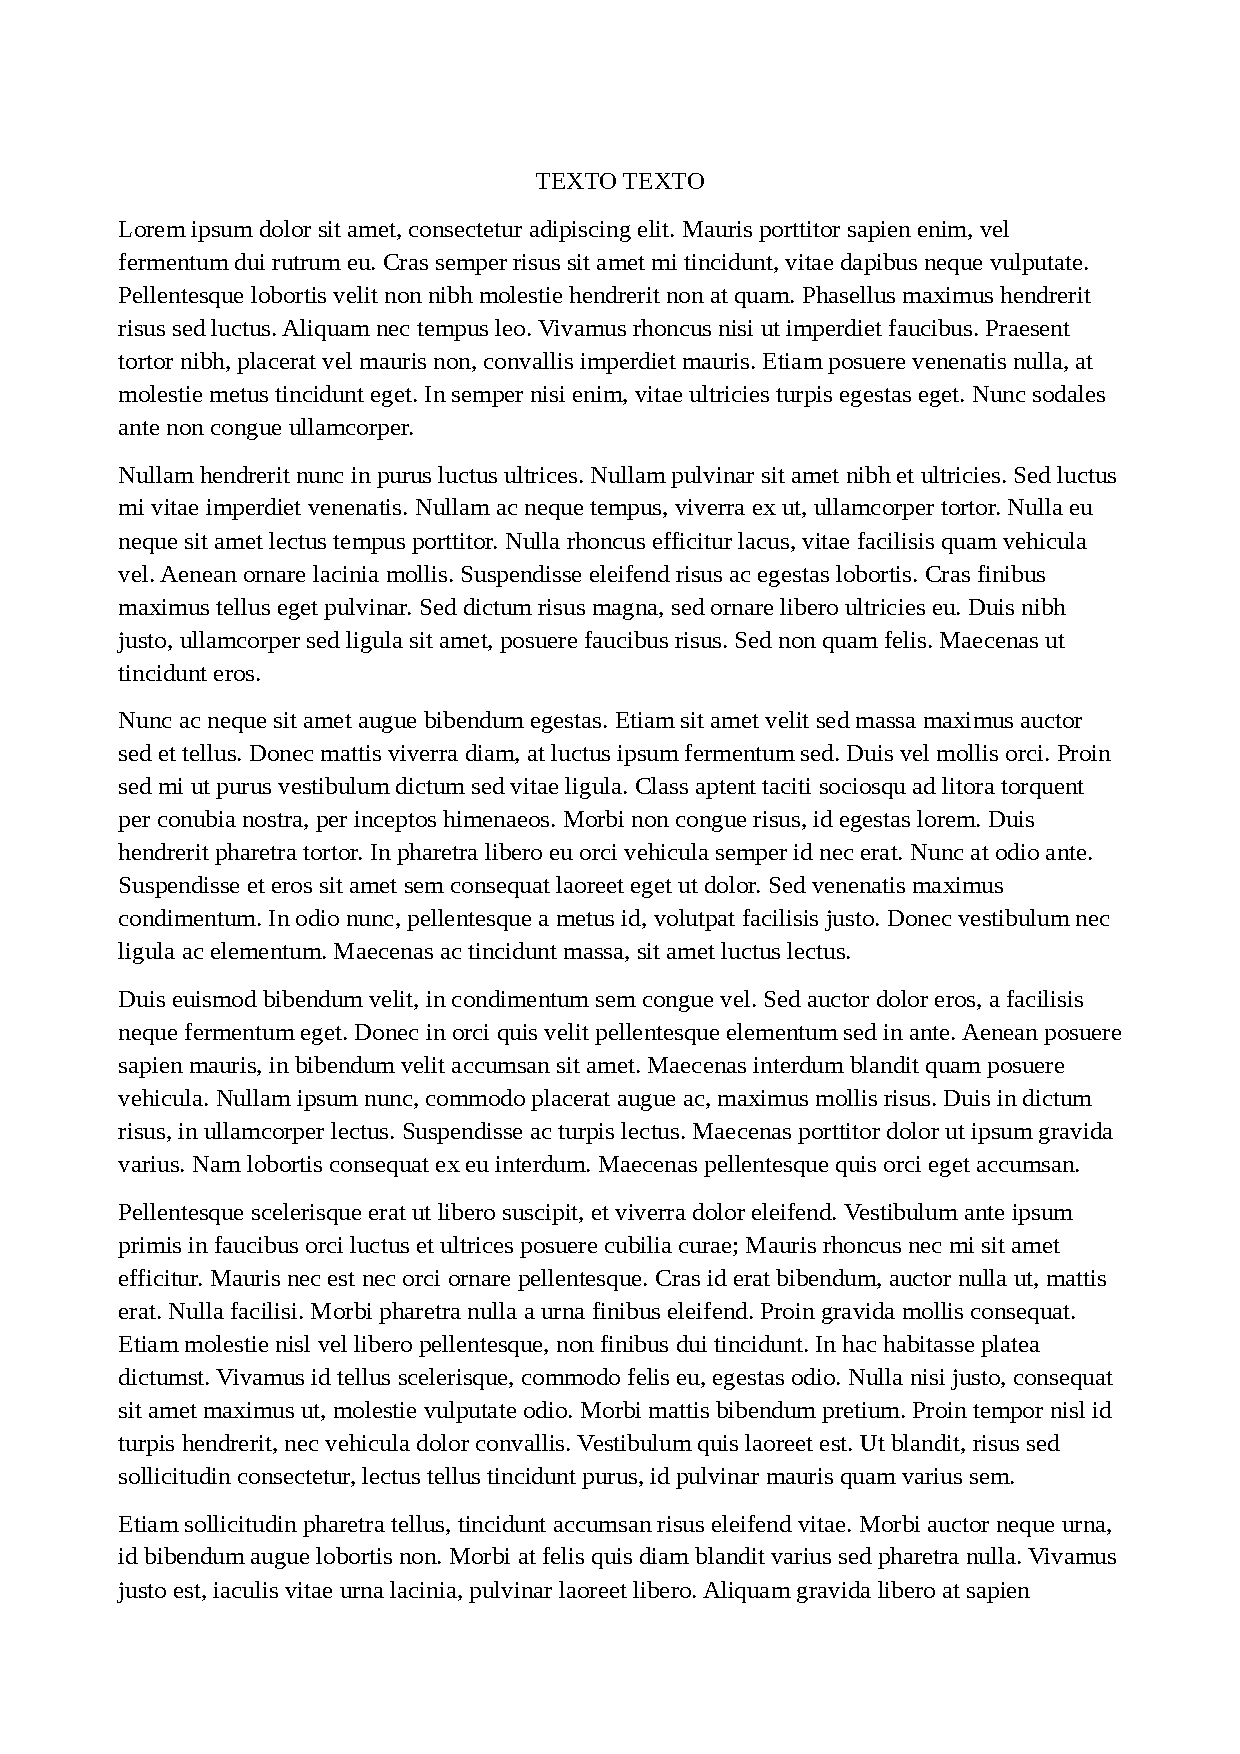
\includepdf[pages={1},scale=0.80,pagecommand=\chapter{Texto Texto}\label{apen:apendiceC}]{appendix/apendiceC}
\includepdf[pages={2},scale=0.80,pagecommand={}]{appendix/apendiceC}


\addtocontents{toc}{\endgroup}
\end{apendicesenv}



 % apendice
	
% ----------------------
% força para que não exiba subtítulos em apêndices no sumário
% -----------------------

\begin{anexosenv}
\addtocontents{toc}{\protect\setcounter{tocdepth}{1}}
\makeatletter
\addtocontents{toc}{%
  \begingroup
  \let\protect\l@chapter\protect\l@section
  \let\protect\l@section\protect\l@subsection
}
\makeatother
% Imprime uma página indicando o início dos apêndices
% \partapendices

%coloca o identificador do anexo/apendice somente na primeira página
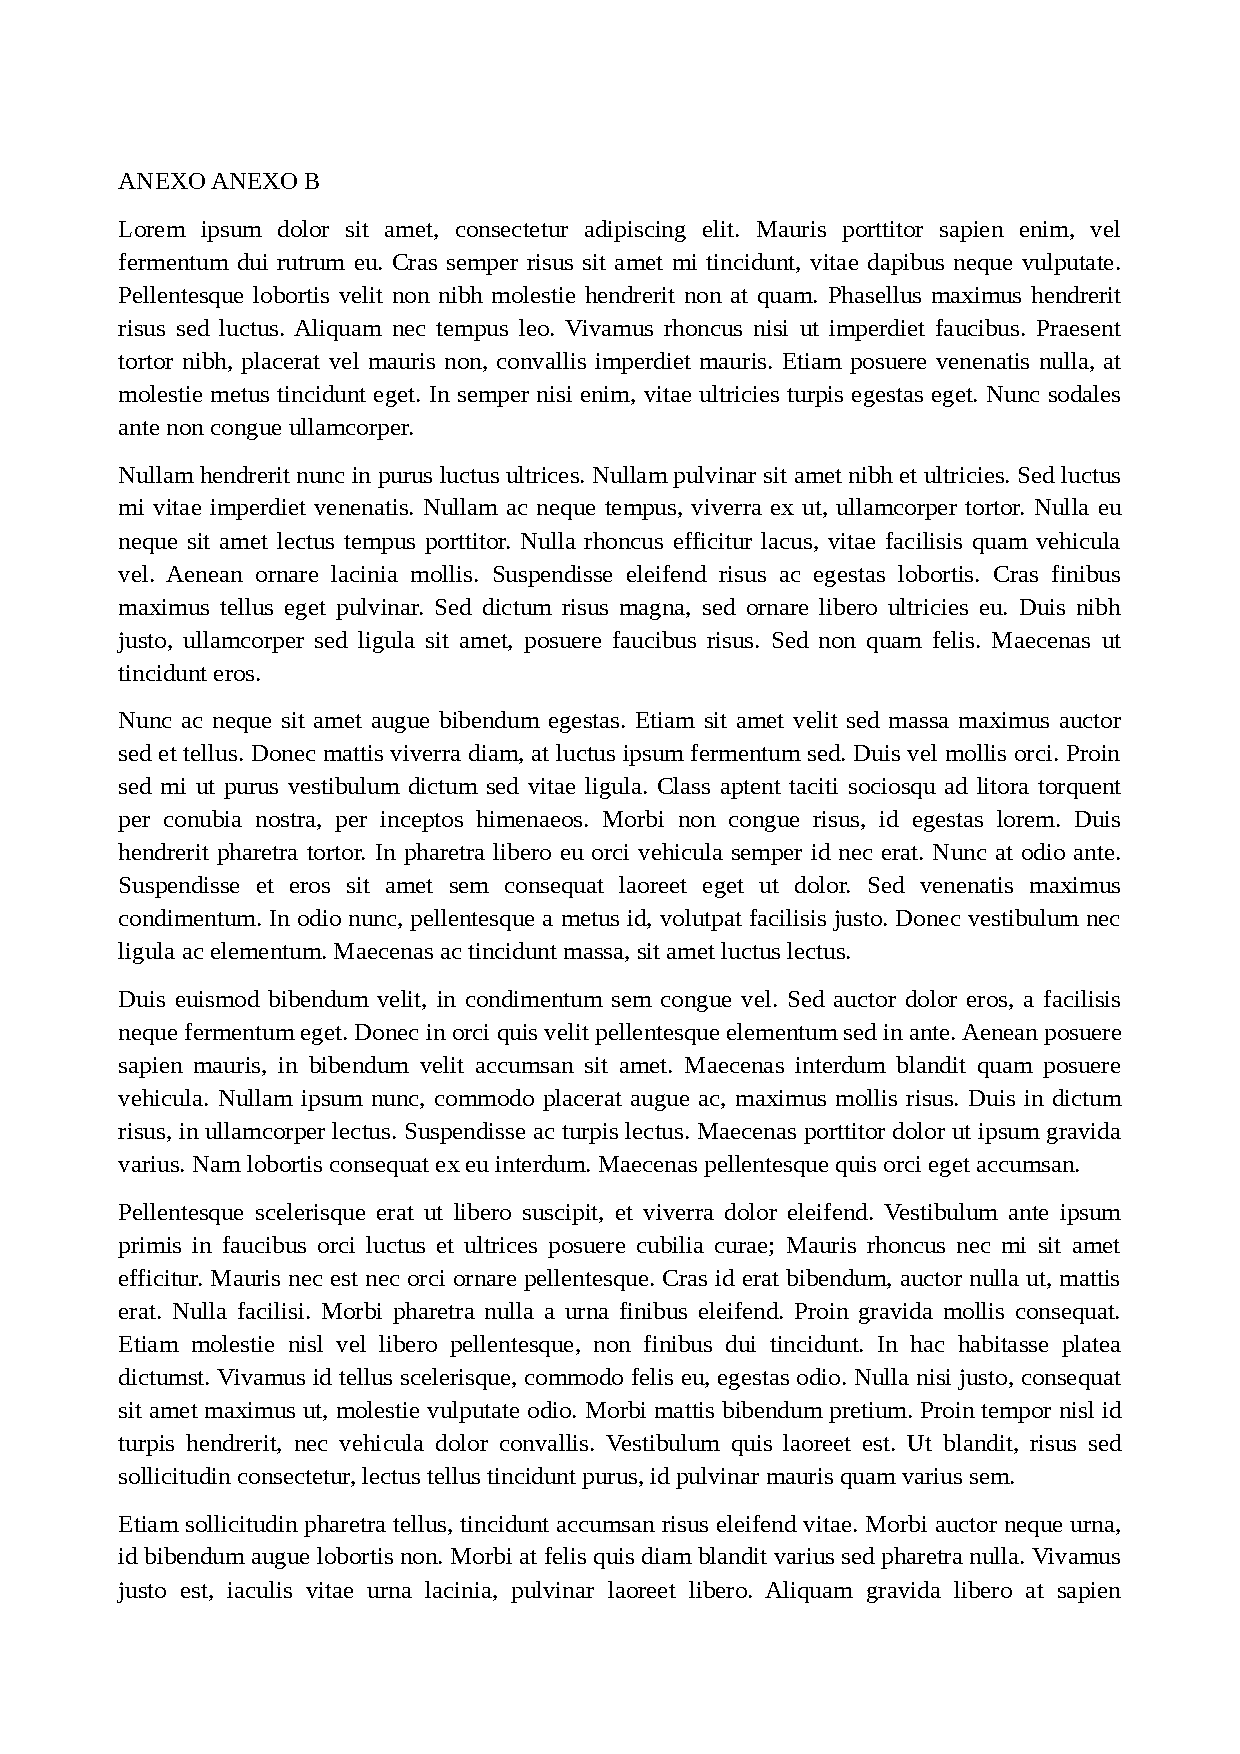
\includepdf[pages={1},scale=0.8,pagecommand=\chapter{Texto Texto Texto Texto}\label{anex:anexob}]{anexos/anexoB}
\includepdf[pages={2-},scale=0.80,pagecommand={}]{anexos/anexoB}

%coloca o identificador do anexo/apendice somente na primeira página
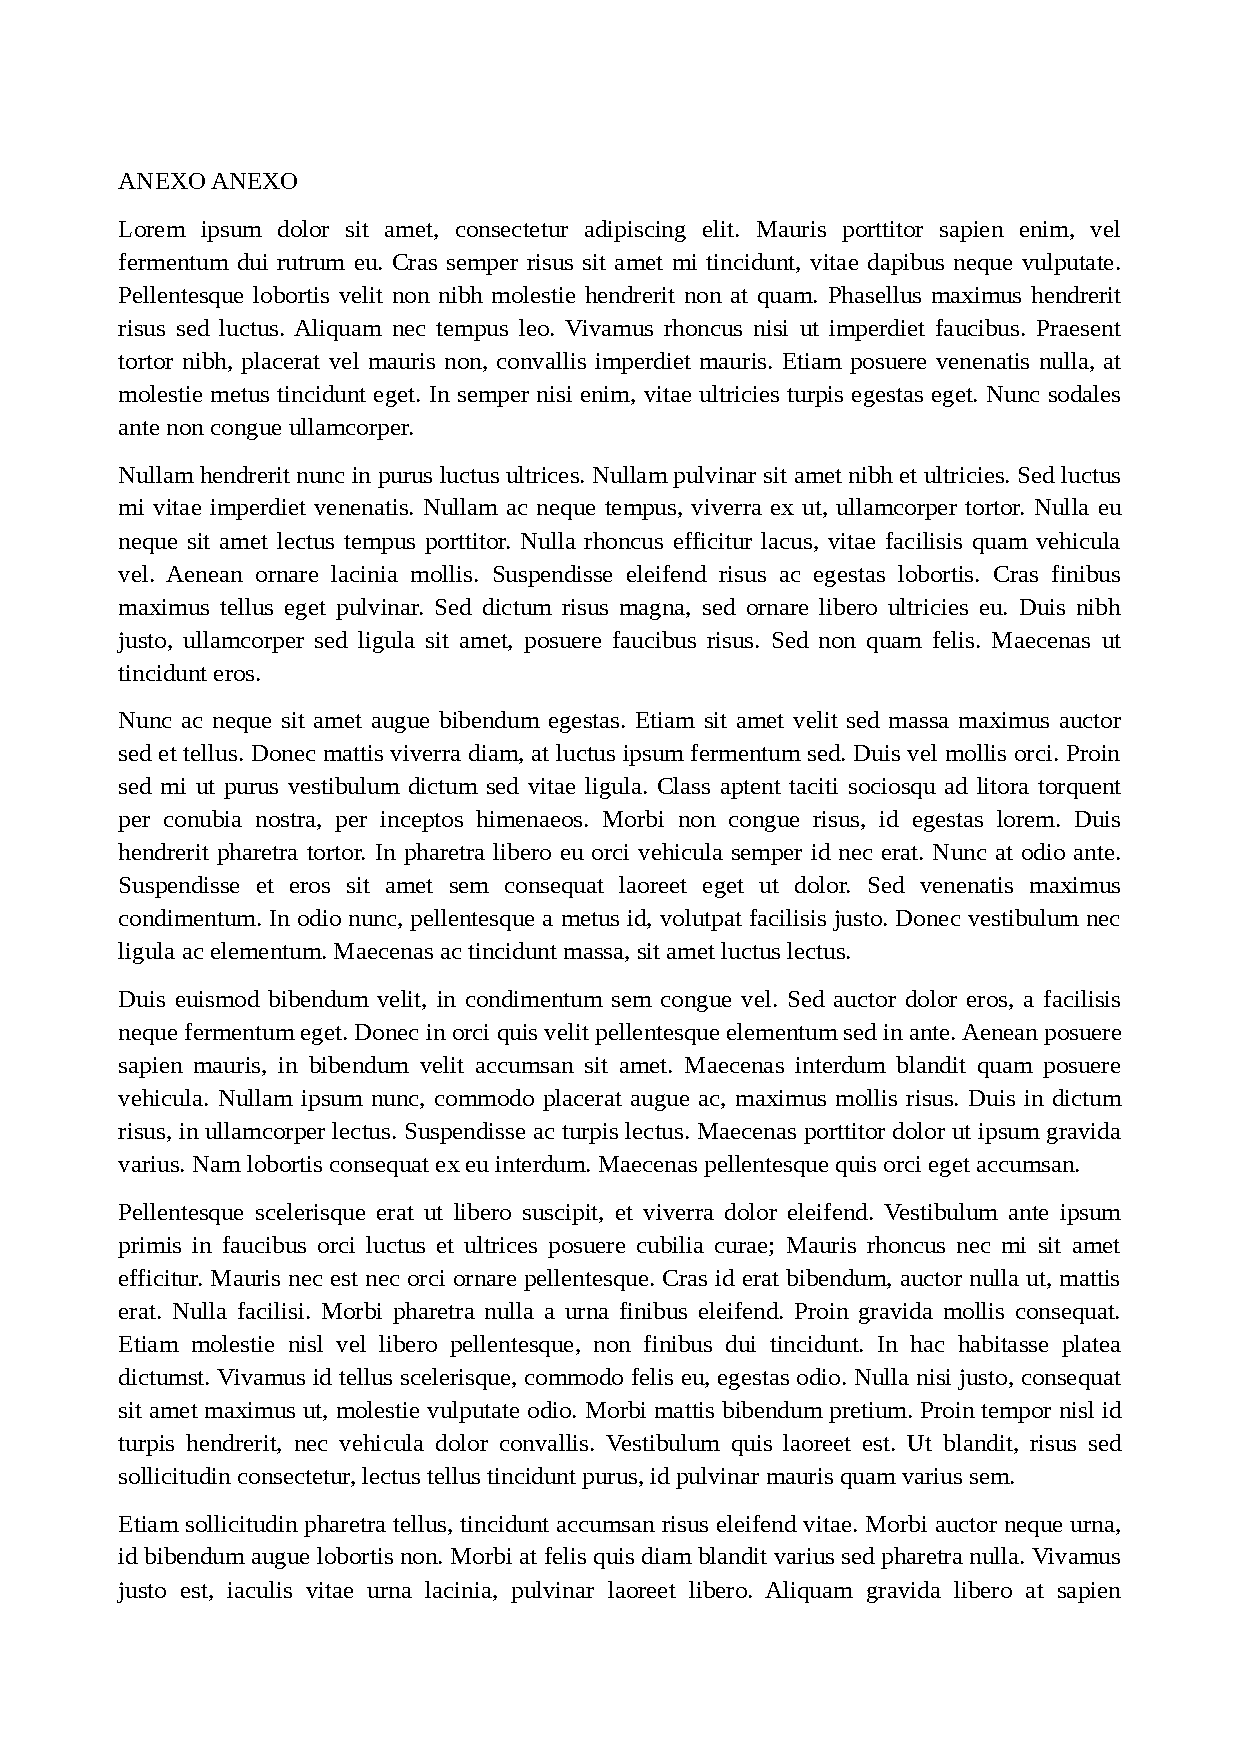
\includepdf[pages={1},scale=0.8,pagecommand=\chapter{Texto Texto Texto Texto}\label{anex:anexoa}]{anexos/anexoA}
\includepdf[pages={2-},scale=0.80,pagecommand={}]{anexos/anexoA}

\addtocontents{toc}{\endgroup}
\end{anexosenv}



 % anexos
%	
\newglossaryentry{naive-bayes}
{
  name=\textit{Na{\"i}ve Bayes},
  description={},
  plural=\textit{Na{\"i}ve Bayes}
}

\newglossaryentry{hoeffding-tree}
{
  name=\textit{Hoeffding Tree},
  description={},
  plural=\textit{Hoeffding Trees}
}












 % glossario

\printindex


\end{document}
